\chapter{Theory}
\label{cha:theory}

In this chapter the theory behind the techniques used in this thesis work will be presented.
The first section will treat supervised text classification, which will act like a foundation for the active learning that will come after.
Active learning is the main focus of the chapter, and an overview of the field as well as some concrete techniques will be covered.
The techniques covered will mainly be in regards to multi-labeled data.
In addition to this, some unsupervised methods used in the data processing will be covered.
This chapter will then end by going through the different evaluation metrics that will be use to assess the methods used.

Most of this Chapter deals with text data.
Before using the techniques presented in this chapter, the text need to be represented in a way that is easy to work with.
\textit{Bag-of-words} (BoW) is one of the more common representations when performing text analysis. 
Using BoW the text is represented as a multi-set, a document is represented by the number of occurrences of the different words. 
Like the name implies, the positions of the words are not taken into account, they are viewed as if they were taken from a bag. 
One way to incorporate positional information into the representation is the use of n-grams.
Instead of storing information pertaining to one term, information is stored with regards to n consecutive terms.
Consider the text ``Pattern Recognition and Machine Learning''.
The use of an n-gram with n=2, called a bigram, would result in the tokens: ``Pattern Recognition'', ``Recognition and'', ``and Machine'', and ``Machine Learning''.

\section{Text Classification}\label{sec:text-classification}

The problem in text classification is to assign one or more classes to a given text document~\cite{aggarwal2012surveyclass}.
It is mainly approached with supervised machine learning.
That is, with a dataset that consists of a collection of text documents, where each document has one or more classes assigned to it.~\cite{bishop2006pattern}.
With the help of these labels, a classification model is fitted to the data.
The goal of this is for the model to be able to correctly assign a class to a a previously unseen text document.
Some of these classification models can also produce a probability of a document being of a certain class.
Other models are based on the concept of a margin that separates the classes, and the distance between a data point and a margin can be used to indicate how certain the model is of the assigned label~\cite{tong2001support}.
Example of use cases for text classification is categorization of news articles, document retrieval and email filtering.
There exist several different models for classifying text.
Decision trees, neural networks and Support Vector Machines (SVM) are some have been previously applied to the text domain with successful results~\cite{aggarwal2012survey}.
In this thesis, SVM are the main focus, since they have been studied extensively in the context of active learning~\cite{tong2001support, settles2012active, brinker2006active, yang2009effective}.
Logistic regression is used for the binary classification task of identifying invalid reports. %TODO: Refer to proper thing

\subsection{Support Vector Machines}

SVMs work by implicitly map the training data to a feature space~\cite{bishop2006pattern}.
The goal is that the data should be linearly separable in the feature space, even if it is not in the input space.
In the case of binary classification, a point is classified by the linear model:
\begin{equation}\label{eq:svm-y}
    y(x) = w^T \phi(x) + b
\end{equation}
where the sign of $y(x)$ determines which label will be assigned to $x$.

The goal of an SVM is to try to find the hyperplane that maximizes the margin.
That is, the distance between any point and the decision boundary should be as large as possible.
A subset of the data points will be used to determine where the decision boundary is, these points are called the support vectors.
The hyperplane that gives us the maximum margin can be found by:

\begin{equation}
    \argmin_{w}\frac{1}{2}||w||^2
\end{equation}

In order to allow for better generalization, and for data that is not completely linearly separable, SVMs make use of slack variables, denoted $\xi_n$.
The slack variables are intended to penalize points that are close to the decision boundary~\cite{bishop2006pattern}.
A parameter $C>0$ controls how much effect the slack variables will have.
The equation with the slack variables becomes:

\begin{equation}
    \argmin_{w}\frac{1}{2}||w||^2 + C \sum_n\xi_n.
\end{equation}

A smaller $C$-value allows more points to be misclassified, which is done in order to achieve better generalization.

\subsubsection{Logistic Regression}

Despite having regression in the name, logistic regression is a classification model.
It is appropriate to use when there are categorical, binary, targets.
Logistic regression works by determining the conditional probability of a class $C_1$, given a feature vector $\phi$.
This probability can then be used with a certain threshold to determine whether or not a data point is a part of a certain class.
Consider the case where we have two classes, $C_1$ and $C_2$.
Their probabilities are then calculated by~\cite{bishop2006pattern}:
\begin{equation}\label{eq:logistic-regression}
    p(C_1|\phi) = sigm(w^T\phi)
\end{equation}
where $sigm$ is the \textit{logistic sigmoid} function defined as:

\begin{equation}
    sigm(a) = \frac{1}{1+e^{-a}}
\end{equation}

The probability for $C_2$ is then obtained with:

\begin{equation}
    p(C_2|\phi) = 1 - p(C_1|\phi)
\end{equation}

From Equation~\ref{eq:logistic-regression} it is clear that the number of parameters in the model is the same as the number of dimensions in the feature vector.
Maximum likelihood is used in order to determine the values of these parameters.
For a dataset with the features $x_n$ for $n=1,...,N$ and targets $t_n \in \{0,1\}$, the likelihood function can be written as:
\begin{equation}
    p(\boldsymbol{t}|w) = \prod_{n=1}^N P(C_1|\phi)^{t_n}(1-y_n)^{1-t_n}
\end{equation}
where $\boldsymbol{t} = (t_1, ..., t_N)^T$.

This is traditionally used with the Iterative Reweighted Least Squares method~\cite{bishop2006pattern}.

\subsection{Multi-Label Classification}\label{subsec:multi-label-classification}

Multi-label classification is the type of text classification where one instance can be associated with multiple labels.
It is a generalized version of the multi-class classification problem, where there is more than 2 labels, but each document is only assigned one~\cite{tsoumakas2006multi}.

A common way of solving multi-label classification problems is the Binary Relevance method~\cite{read2011classifier, boutell2004learning, luaces2012binary}.
It is a way of transforming the multi-label classification problem into several different binary ones.
With Binary Relevance one classification model per label is fitted on the data.
Each of these classifiers are then predicting whether or not the document is associated with the corresponding label or not.

\section{Active Learning}\label{sec:active-learning}

Conventional machine learning systems use a set of available data to find a hypothesis that can explain the patterns within the data.
The purpose of active learning is to allow a system to select the data that it wants to be labeled, and therefore the data it wants the model to be trained on~\cite{settles2012active}.
An active learning system samples a document to be labeled from a pool of unlabeled data.
With this sample an oracle, which is often a human annotator, is then queried to get the label for that document.
By being able to decide what data to label and use, the goal is that the system can achieve better results, and that the training data will be of higher quality.
To get a better understanding of how the process works, these are the steps that are commonly iterated over until enough samples have been labeled:
\begin{enumerate}
    \item Evaluate the samples in the unlabeled pool based on a particular measure that is defined by the sampling strategy.
    \item The selected samples are presented to an oracle that is queried for the labels. This oracle is commonly in the form of a human annotating the instances. \label{enum:label}
    \item The newly labeled samples are added to the labeled pool.
    \item A machine learning model is trained on the labeled pool, this model is often used by the sampling strategy in order to select samples to label in step~\ref{enum:label}
\end{enumerate}
A model of the active learning system can be seen in Figure~\ref{fig:active-learning-model}.

In several different domains, data is readily available and easy to obtain.
But even if the data is abundant, labels for the data are often harder and more expensive to come by, especially when it comes to multi-label problems~\cite{settles2012active}.

In Section~\ref{sec:pool-based-sampling} different ways to access the data in active learning are described
This is followed by some theory of how the samples relate to the hypothesis space, in Section~\ref{sec:the-version-space}.
The active learning theory then ends with a description of three multi-label active learning strategies.

\subsection{Pool-Based Sampling}
\label{sec:pool-based-sampling}

The main focus in active learning is how to select the samples to be labeled.
There are different sampling methods in use, and which one is more appropriate depends on how the data can be accessed.
Pool-based sampling is motivated by the assumption that there exist a large available pool of data, where only a small portion is labeled~\cite{lewis1994sequential, settles2012active}.
The samples to be labeled are selected by evaluating the entire pool of unlabeled data, and choosing the most appropriate ones based on a defined utility measure.
If the entire pool is too large, a subset could be used instead.
For applied active learning, pool-based sampling seems to be the most popular choice~\cite{li2013active}, but there are some alternatives that have been used in theoretical settings such as stream-based selective sampling.
The difference between stream-based selective sampling and pool-based sampling is that the draws one sample at a time from an input source and make the decision whether or not to query a label for it.
For text applications, where a set of data is often readily available, pool-based sampling is often the more appropriate option since the entire dataset can be considered.
Pool-based is therefore the sampling technique that is considered in this thesis.

\subsection{The Version Space}
\label{sec:the-version-space}

In machine learning, a hypothesis is a specific configuration of a model, the purpose of which is to predict outputs on new instances of data by generalizing the training data.
One hypothesis can, for example, be an SVM model with specific values for the parameters.
The set of all possible hypothesis that we are working with is called the \textit{hypothesis space}, denoted $\mathcal{H}$~\cite{russell2016artificial}.
Following the SVM example, the hypothesis space would be the set of SVMs with the different parameter values under consideration.
The subset of the hypothesis space that in the feature space separates the data is called the version space, which is defined as~\cite{settles2012active,tong2001support}:

\begin{equation}\label{eq:version-space}
    \mathcal{V} = \Big \{ f \in \mathcal{H} \Big | y_i f(x_i) > 0, \forall i \in \{i \dots n\} \Big \}
\end{equation}
When the assigned label $y_i$, and the predicted label $f(x_i)$ has the same sign, $y_i f(x_i)$ will be positive, and therefore included in $\mathcal{V}$.

So the version space therefore represents the different hypotheses that make correct predictions on the training data.
Under the assumption that one of the hypothesis can fully separate the data, the version space shrinks when more labeled data is acquired.
So for new labeled instances the hypotheses in the version space will give better predictions for the training data.
Based on this, an active learning algorithm should aim to reduce the size of the version space with each new sample. 
Optimally the selected sample should cut the version space in half in each iteration.
By doing this it can be viewed as a sort of binary search, looking for the hypothesis that can fully separate the data.

There exists a useful relationship between the feature space $\mathcal{F}$ and the hypothesis space $\mathcal{H}$ called the \textit{version space duality}~\cite{tong2001support, vapnik1998statistical}.
It states that hyperplanes in the hypothesis space corresponds to points in the feature space, and the other way around.
So by selecting points to be labeled, constraints can be enforced on the hypothesis that form the version space.

One approach to this that has shown to be successful is \textit{uncertainty sampling}~\cite{settles2012active}.
This is commonly done with SVM, since the idea behind SVM is to find a hyperplane that separates two classes in a binary classification with the maximum margin.
Out of the different hyperplanes in the hypothesis space, the version space contains those that can successfully separate the data.
Uncertainty sampling aims to select the points in the feature space that will reduce the amount of the valid hypotheses the most.
An SVM model tries to find the support vectors that maximizes the decision boundary in the feature space, separating the two classes.
Considering this in $\mathcal{H}$, it will be analogous to the hypothesis in the center of the hypothesis space, which is encompassed by the constraints set by the labeled data.
What uncertainty sampling predicts are the values for the unlabeled points, and then choosing the one that it is most uncertain about.
The selected sample will therefore be the sample closest to the decision boundary of the SVM.
Based on the version space duality, it is a good approximation for dividing the version space in two~\cite{settles2012active}.

\subsection{Binary Version Space Minimization}\label{subsec:binmin}

Binary version space minimization (BSVM) is a generalization of uncertainty sampling, that is designed to make it work with multi-label data.
The approach taken is to decompose the multi-label problem to several binary tasks with the binary relevance method, as is discussed in Section~\ref{subsec:multi-label-classification}.
The unlabeled point that is chosen for labeling is then the one with the smallest SVM margin across all the binary classification tasks.
By doing this, it does not incorporate the multiple labels into the decision process, but treats all classes individually and equally. 
Selecting a new data $x_{new}$ to be labeled using BSVM can formally be defined as:
\begin{equation}
    x_{new} = \arg\min_{x \in D_U} \big( \min_{i \in \{1 \dots n\}} y_i(x) \big)
\end{equation}
where $n$ is the number of labels, $y_i(x)$ is the function from Equation~\ref{eq:svm-y} for the binary SVM classifier that is used to predict label $i$, and $D_U$ is the set of unlabeled data points.

\subsection{Maximum Loss Reduction with Maximum Confidence}\label{subsec:mmc}

Maximum loss reduction with maximum confidence (MMC) was developed by Yang et al~\cite{yang2009effective}.
The goal of this technique is to find the samples that will reduce the expected model loss the most, and select this sample for labeling.
These are the basic notations that will be used when explaining the MMC approach:
\begin{itemize}
    \item The labeled dataset: $D_L$.
    \item The unlabeled dataset: $D_U$.
    \item Possible query set: $D_S$.
    \item Optimal query set: $D^*_S$.
    \item The classification function that is trained on dataset $D_L$: $f_{D_L}$.
    \item A data point: $x$, and its label: $y$.
    \item The loss of on data point $x$: $L(f_{D_l}(x))$.
    \item The expected loss of the model: $\widehat{\sigma_{D_L}}$.
\end{itemize}

The expected model loss that MMC is trying to reduce can be defined as follows~\cite{yang2009effective}:
\begin{equation}
    \widehat{\sigma_{D_L}} = \int_x \bigg ( \sum_{x \in Y} L(f_{D_L})P(y|x) \bigg ) P(x)dx
\end{equation}

It is hard to estimate $P(x)$, so it is instead measured over all the samples in $D_U$.
This results in the estimate:
\begin{equation}
    \widehat{\sigma_{D_L}} = \frac{1}{|D_U|} \sum_{x \in D_U} \sum_{y \in Y} L(f_{D_L})P(y|x)
\end{equation}

After a set of data points $D_S$ has been labeled, the new dataset $D'_L=D_L + D_S$ is obtained.
Under the assumption that any $x \in D_U - D_S$ has an equal effect on a model trained on the datasets $D_L$ and $D'_L$, we get the following equation for the reduction of the expected loss~\cite{yang2009effective}:

\begin{equation}
    D^*_S = \arg\max_{D_S}(\widehat{\sigma_{D_L}} - \widehat{\sigma_{D'_L}}) = \arg\max_{D_S} \big ( \sum_{x \in D_S} \sum_{y \in Y} (L(f_{D_L}) - L(f_{D'_L})) P(y|x) \big )
\end{equation}

In their paper, Yang et al\@.~\cite{yang2009effective} considers the process of finding the greatest reduction in two steps: finding a good estimate for the conditional probability $p(y|x)$, and finding a way to assess the loss reduction of a multi-label classifier.

It is unfeasible for a query strategy to provide a an estimation for all possible label combinations.
If there are $n$ different labels, there will be $2^n$ different label combinations.
In order to estimate the conditional probability $p(y|x)$, MMC uses an approach that first estimates the number of labels for a given data point, and then uses that estimate to select the most probable labels.
Consider the case where a data point has $m$ labels.
By obtaining the probability from our classification model for each label we can sort them in descending order.
If the sample has $m$ labels, then those should the the first $m$ ones in the sorted list.
Furthermore, the probabilities for these $m$ labels are probably significantly higher than the probabilities for the labels that follow.
There should be a clear separation between them.

Yang et al\@.~\cite{yang2009effective} describe the process of estimating the number of labels as follows:
\begin{enumerate}
    \item Use the classification model to obtain the probabilities for each label for all the data samples.
    \item For each data sample, sort and normalize the probabilities for all the labels.
    \item Using the labeled dataset, fit a logistic regression classifier with the sorted and normalized probabilities as features, and the number of labels as target.
    \item With the fitted logistic regression model, predict the number of labels for the samples in the unlabeled pool.
\end{enumerate}

After obtaining the predicted number of labels $m$ for a sample $x$, the estimate for $p(y|x)$, denoted $\hat{y}$, is then obtained by selecting $m$ the most probable labels based on the original classification models output.

now the loss for the multi-label classifier needs to be defined.
By using the model where there are $k$ different binary classifiers for a problem with $k$ labels, the model loss can be calculated by adding the loss for the different binary classifiers like:
\begin{equation}
    L(f) = \sum_{i = 1}^k L(f^i)
\end{equation}
where the loss of a single binary classifier is denoted as $L(f^i)$.
With this definition, it remains to define the measure of loss on a single binary classifier.
The measurement that is used by MMC is to estimate the model loss by the size of the version space of the SVM~\cite{tong2001support, yang2009effective}.
The version space's size can be computed with Equation~\ref{eq:version-space}.
However, computing this for each possible label combination is expensive.
By using the heuristic from~\cite{tong2001active}, an approximation of the version space with the added label can be obtained from the current SVM classifiers' margin.
The reduction rate after adding the data point $(x, y^i)$, where $y^i \in {-1, 1}$, can be expressed as follows~\cite{yang2009effective, tong2001active}:

\begin{equation}\label{eq:reduction-rate}
    \frac{L(f^i_{D_L+(x, y^i)})}{L(f^i_{D_L})} \approx \frac{V^i_{D_L + (x, y^i)}}{V^i_{D_L}} \approx \frac{1 + y^i f^i_{D_L}(x)}{2}
\end{equation}

$L(f^i_{D_L})$ does not involve the sample selected for labeling, so by writing the loss reduction as in Equation~\ref{eq:mmc-loss-reduction} it can be seen that focusing on the reduction rate is sufficient.
\begin{equation}\label{eq:mmc-loss-reduction}
    \begin{split}
        L(f_{D_L}) - L(f_{D'_L}) = \sum_{i=1}^k\big ( L(f^i_{D_L}) - L(F^i_{D'_L}) \big )\\
        = \sum_{i=1}^k\big ( L(f^i_{D_L}) \dot (1 - \frac{L(F^i_{D'_L})}{L(F^i_{D_L})}) \big )
    \end{split}
\end{equation}
By incorporating the result from Equation~\ref{eq:reduction-rate}, the following approximation for the reduction rate is obtained:
\begin{equation}
    \sum_{i=1}^k\big ( \frac{1 - y^if^i_{D_L}(x)}{2} \big )
\end{equation}

The only thing that remains is now to combine the estimation of $p(x|y)$ with the estimate for loss reduction.
The resulting equation, called maximum loss reduction with maximal confidence, is~\cite{yang2009effective}:

\begin{equation}
    D^*_S = \arg \max_{D_S} \big ( \sum_{x \in D_S} \sum_{i=1}^k (\frac{1 - \hat{y}^if^i_{D_L}(x)}{2}) \big )
\end{equation}

The full algorithm for the approach can be seen in Algorithm~\ref{alg:mmc}.

\begin{algorithm}
    \begin{algorithmic}
        \REQUIRE Labeled set $D_L$\\
                 Unlabeled set $D_U$ \\
                 Number of classes $k$ \\
                 Number of selected examples per iteration $S$
        \REPEAT
            \STATE Train $k$ binary SVM classifiers $f^1$, \dots, $f^k$ based on training data $D_L$.
            \FOR{each $x \in D_U$ \textbf{do}}
                \STATE Predict its label vector using the method described in Section~\ref{subsec:mmc}.
                \STATE Calculate the expected loss reduction with the most confident label vector $\hat{y}$, $score(x) = \sum_{i=1}^k (\frac{1 - \hat{y}^if^i_{D_L}(x)}{2})$
            \ENDFOR
            \STATE Sort $score(x)$ in decreasing order for all $x$ in $D_U$.
            \STATE Select a set of $S$ examples $D_S^*$ with the largest scores, and update the training set $D_L \Leftarrow D_L + D^*_S$.
        \UNTIL{enough instances are queried}
    \end{algorithmic}

    \caption{Maximum Loss Reduction with Maximal Confidence procedure. Taken from Yang et al\@.~\cite{yang2009effective}, with some modifications to the notations used in order to make it coherent with the rest of the report.}
    \label{alg:mmc}
\end{algorithm}


\subsection{Adaptive Active Learning}\label{subsec:adaptive-active-learning}

In their paper, Li et al\@.~\cite{li2013active} present two approaches to active learning:
\begin{itemize}
    \item Max-Margin Uncertainty Sampling
    \item Label Cardinality Inconsistency 
\end{itemize}
These two techniques are then combined in a weighted fashion into what they call Adaptive Active Learning (AAL).

\subsubsection{Max-Margin Uncertainty Sampling}

The idea behind \textit{Max-Margin Uncertainty Sampling} comes from the observation that multi-label classification prediction is mainly about separating the positive labels from the negative labels~\cite{li2013active}.
That is, separating the labels are assigned to an instance and the ones that are not.
In order to model the uncertainty of the prediction on a datapoint, Li et al\@. suggest the usage of a global separation margin to separate the negative labels from the positive.

The positive labels for a data point $x$ is defined as those where $sign(f'_{D_L}(x))$ is positive.
The separation margin is defined as:
\begin{equation}
    \begin{split}
        sep\_margin(x) = \min_{i \in \hat{y}^+}|f'_{D_L}(x)| + \min_{i \in \hat{y}^-}|f'_{D_L}(x)|
    \end{split}
\end{equation}
where $\hat{y}^+$ denotes the set of predicted labels that are positive on the instance, and the $\hat{y}^-$ denotes the negative ones.

The data point that the model is the most uncertain about is then the one with the smallest margin.
Li et al\@. define their global measure, max-margin prediction uncertainty, as:
\begin{equation}
    u(X) = \frac{1}{sep\_margin(X)}
\end{equation}

\subsubsection{Label Cardinality Inconsistency}

\textit{Label Cardinality Inconsistency} is based on the assumption that the underlying distribution is the same for the labeled and unlabeled data.
In a multi-label dataset, the \textit{label cardinality} is defined as the average number of labels assigned to each class~\cite{tsoumakas2006multi}.
The selection strategy that Li et al\@. based on this measures the Euclidean distance between the number of assigned predicted labels on $x$, and the label cardinality of the labeled data:
\begin{equation}
    c(x) = \bigg \lVert \sum_{i \in \hat{y}^+} 1 - \frac{1}{N_L} \sum_{y \in Y_L} \sum_{i \in y^+} 1 \bigg \rVert_2
\end{equation}
where $N_L$ is the number of labeled samples, $Y_L$ are the labels for those samples, and $y^+$ are the positive labels in $y$.

\subsubsection{Integration - Adaptive Active Learning}

Since \textit{max-margin uncertainty sampling} and \textit{label cardinality inconsistency} complement each other, an integration method is used:
\begin{equation}\label{eq:approx-generalization-error}
    q(x, \beta) = u(x)^\beta \cdot c(x)^{1-\beta}
\end{equation}
where $\beta$ is a parameter controlling the weight put on the two measures.
This parameter is chosen by in each iteration evaluating a discrete set of values, for example $\{0, 0.1, 0.2, \dots, 1\}$.
The selection of $\beta$ is then based on the most informative sample amongst them.
Equation~\ref{eq:approx-generalization-error} shows the \textit{approximate generalization error}, which is used to select the sample.
\begin{equation}\label{eq:calc-epsilon}
    \epsilon(x) = \sum_{x \in D_U} \max_{i \in f(x)^+}(1-f^i(x)) + \max_{i \in f(x)^-}(1+f^i(x))
\end{equation}
,where $f(x)^+$ and $f(x)^-$ are the predicted positive labels, and negative labels, respectively.
So, the sample is then selected by:
\begin{equation}\label{eq:x-star}
    x^* = \arg \min_{x \in D_U} \epsilon(x)
\end{equation}

The complete algorithm for the integrated approach can be seen in Algorithm~\ref{alg:adaptive-active-learning}.

\begin{algorithm}
    \begin{algorithmic}
        \REQUIRE Labeled set $D_L$ \\ 
                 Unlabeled set $D_U$ \\ 
                 Parameter set $B$
        \REPEAT
            \STATE Train multi-label SVM classifier $F^0$ on $D_L$.
            \FOR{each $x_i \in D_U$ \textbf{do}}
                \STATE Compute $u(x_i)$ and $c(x_i)$.
            \ENDFOR
            \FOR{each $\beta \in B$ \textbf{do}}
                \STATE Mark a candidate instance $x = \arg\max_{x \in D_U} q(x, \beta)$
            \ENDFOR
            \STATE Copy all marked candidate instances into a set $S$.
            \FOR{each $x \in S$ \textbf{do}}
                \STATE Produce $\hat{y}$ using classifier $F^0$.
                \STATE Retrain a new classifier $F$ on $(x, \hat{y}) \cup D_L$.
                \STATE Compute $e(x)$ using classifier $F$ and Equation~\ref{eq:calc-epsilon}.
            \ENDFOR
            \STATE Select instance $x^*$ from $S$ using Equation~\ref{eq:x-star}
            \STATE Remove $x^*$ from $D_U$, query its label vector $y^*$.
            \STATE Add $(x^*, y^*)$ to $D_L$.
        \UNTIL{enough instances are queried}
    \end{algorithmic}

    \caption{AAL Procedure. Taken from Li et al\@.~\cite{li2013active}, , with some modifications to the notations used in order to make it coherent with the rest of the report.}
    \label{alg:adaptive-active-learning}
\end{algorithm}


\section{Text Processing using Unsupervised Techniques}

Techniques in machine learning that do not require a set of categorized data is called unsupervised learning.
They use the structure of the data to obtain the information to use when processing it.
These techniques may have different goals.
Some are used to estimate a distribution, others are used to reduce the number of dimensions in the data by trying to find dimensions that capture as much as possible of the variance, and some are used for the purpose of identifying groups of similar points within the data~\cite{bishop2006pattern}.
When it comes to text data, there are a few common methods and techniques that are unsupervised, and can be used for different purposes.
Examples of such techniques are \textit{topic modeling} and \textit{clustering}.
Another interesting technique is word2vec, that is used to produce word embeddings.

As described in Section~\ref{sec:text-classification}, with BoW a document is represented by the number of occurrences of the different words. 
Representing text in this way therefore becomes high-dimensional, there is one dimension for each word in the vocabulary. 
In written language a word can be used to express several different thoughts, and one thought can be expressed using several different words.
This is something that cannot be captured with BoW.
However, it is easy to work with, and is commonly used when performing topic modeling among other things.

\subsection{Topic Modeling}\label{sec:topic-modeling}

A topic model is a statistical model for finding topics within text~\cite{crain2012dimensionality}.
The topics build upon the probability that a certain word would occur in a text about a given topic, on the basis of terms occurring together.
For example, if the topic represents United States politics, words such as ``government'', ``Trump'', ``Reagan'', ``Senate'', or ``Medicaid'' are more likely to appear than ``sailboat'' or ``sweater''.
Any given document can then contain a certain topic with some probability.
This can be viewed as fuzzy clustering, and that the document has a degree of membership in a topic or cluster~\cite{crain2012dimensionality}.
The most common topic model in use today is Latent Dirichlet Allocation (LDA)~\cite{crain2012dimensionality}.
Another topic model that preceded LDA is Probabilistic latent semantic analysis (PLSA)~\cite{hofmann1999probabilistic}.
However, PLSA has been shown to be more prone to overfitting than LDA~\cite{crain2012dimensionality}.

In the rest of the report, the following notation will be used:

\begin{itemize}
    \item $D$ denotes a corpus of $M$ documents: $D = \{w_1, w_2, \ldots, w_M\}$.
    \item The number of topics is $K$. Each topic is indexed by $i$.
    \item $N_d$ is the number of terms in document $d$.
    \item $N_i$ is the number of terms $n$ in topic $i$.
    \item $V$ denotes the number of words in the vocabulary.
\end{itemize}

\subsubsection{Latent Dirichlet Allocation}

Latent Dirichlet allocation (LDA) is a statistical model, where abstract topics in the model are defined as distributions over words~\cite{blei2003latent}.
LDA is based on a generative process, a model of which can be seen in Figure~\ref{fig:lda_gen_process}.
The circles in this figure represent random variables.
Dependencies between these random variables are shown with arrows, and if a variable is observed it is shaded in the figure.
In this model, the only observed variable is the words in the document.
Parts of the model are surrounded by a rectangle to show that the part is repeated several times.

\begin{figure}
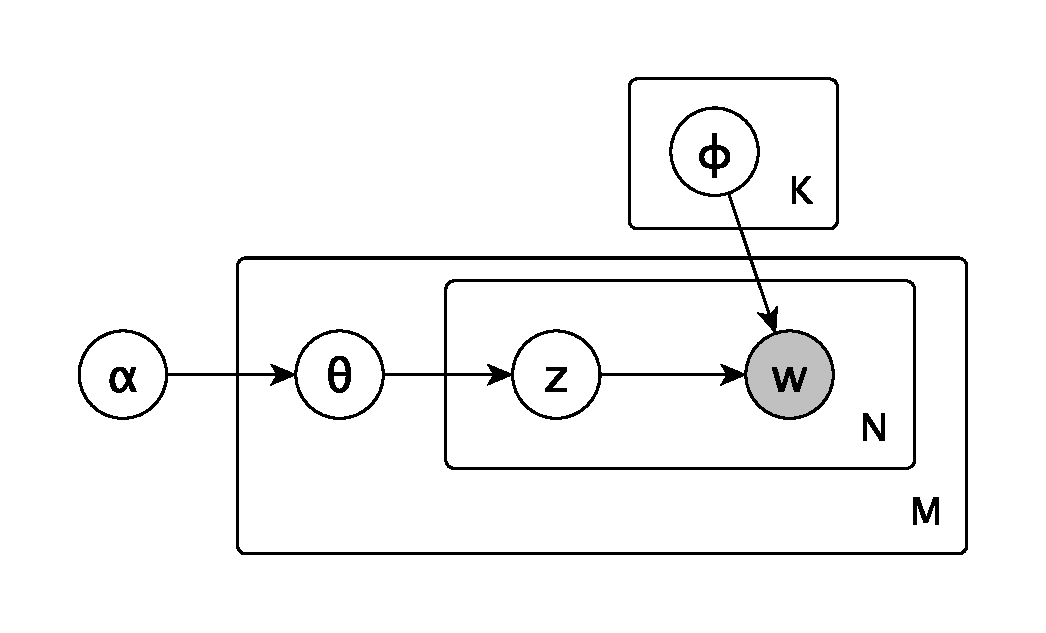
\includegraphics[scale=0.7]{figures/lda-generative-process.eps}
\caption{Diagram of the LDA model.}\label{fig:lda_gen_process}
\end{figure}

The generation of a corpus is done with the following steps~\cite{crain2012dimensionality, blei2003latent}:

\begin{itemize}
    \item \textbf{Draw a distribution over the words for each topic.}
        A sample $\Phi_i$ is drawn from a symmetric Dirichlet distribution with parameter $\beta$. 
        This sample represents the distribution of terms for the topic $i$.

        \begin{equation}
            \Phi_i \sim Dir(\beta)
        \end{equation}

        \begin{equation}
            p(\Phi_i | \beta) = \frac{\Gamma(V\beta)}{{\Gamma(\beta)}^V} \prod^V_{v=1}\phi^{\beta-1}_{iv}
        \end{equation}

        Here, $\Gamma$ is the gamma function, and $\phi_{iv}$ is the value for a word $v$ in the topic $i$.

    \item \textbf{Draw a distribution over the topics for each document.}
        A sample $\theta_d$ is drawn from a Dirichlet distribution with parameters $\alpha$.
        This sample represents the distribution of topics for document $d$.

        \begin{equation}
            \Theta_d \sim Dir(\alpha)
        \end{equation}

        \begin{equation}
            p(\Theta_d | \alpha) = \frac{\Gamma(\sum^K_{i=1}\alpha_i)}{\prod_{i=1}^K\Gamma(\alpha_i)}\prod_{i=1}^K\theta_{di}^{\alpha_i-1}
        \end{equation}

        Here, $\theta_{di}$ is the probability of topic $i$ for document $d$.

    \item For each token with index $n$:

        \begin{itemize}
            \item \textbf{Draw a topic assignment $z_{dn}$ for the token index $n$.} 
                $z_{dn}$ is drawn from the distribution over topics for each document. 
                That is, $z_{dn}$ is drawn from a multinomial distribution using $\theta_d$ as a parameter.

                \begin{equation}
                    z_{dn} \sim Multinomial(\Theta_d)
                \end{equation}

                \begin{equation}
                    p(z_{dn} = i | \Theta_d) = \theta_{di}
                \end{equation}

            \item \textbf{Draw a token $w_{dn}$.}
                The token $w_{dn}$ is drawn from the topic distribution assigned to the index $n$.
                That is, $w_{dn}$ is drawn from a multinomial with parameter $\phi_{z_{dn}}$.

                \begin{equation}
                    w_{dn} \sim Multinomial(\Phi_{z_{dn}})
                \end{equation}

                \begin{equation}
                    p(w_{dn}=v|z_{dn}=i,\Phi_i) = \phi_{iv}
                \end{equation}

        \end{itemize}

\end{itemize}

The LDA model identifies topics from different terms that occur in the same document.
Consider the case where an LDA model has been used to learn a number of topics.
Two terms that frequently occur together are then likely to be in the same topic.
So, if the same word has been used to express different thoughts, and the word has the same probability in two topics, the words that it co-occurs with can be used to differentiate between the different thoughts.

The task of learning the LDA model is a Bayesian Inference problem.
We have several variables that we cannot observe: the word distribution for the topics ($\phi_i$), the topic assignments for the tokens ($z$), and the topic distribution for the documents ($\theta_d$).
The only observed variables are the words in the document.
We have to approximate the posterior distribution using some sampling method, since it cannot be inferred automatically~\cite{blei2003latent}.

There exist a few algorithms that can be used to learn topics for the LDA model. 
Two of these that has shown to be able to extract useful topics from text are \textit{collapsed Gibbs sampling}~\cite{griffiths2004finding} and \textit{variational Bayes}~\cite{blei2003latent}.  
Variational Bayes works by using simple single-variable models to approximate the LDA\@. 
As a consequence, it disregards any dependencies between the variables.

\subsubsection{Collapsed Gibbs Sampling}

Gibbs sampling is a Markov chain Monte Carlo (MCMC) method that is often used to obtain a good estimate for the distribution of a probability model, when it is not feasible to sample the distribution directly~\cite{crain2012dimensionality}.
With the help of a heuristic, or randomly, Gibbs sampling initializes the variables.
During a large number of iterations the variables are then sampled.
When a variable is being sampled, it is conditioned on the others.
In an MCMC fashion, a number of samples are rejected during an initial burn-in period.
This is done in order to get to a state where the points are more representative of the distribution that is estimated.

Griffith et al\@.~\cite{griffiths2004finding} came up with collapsed Gibbs sampling for the LDA model, where $\theta$ and $\phi$ are marginalized out.
The only variable to then be repeatedly sampled is the topic assignment, $z_{dn}$, conditioned on the assignments of the other tokens.

\subsection{Text Clustering}

Cluster analysis is commonly defined as finding groups in a given dataset.
The members of these groups are determined to be similar by a similarity measure~\cite{kaufman2009finding, aggarwal2012survey}.
Text data are sparse, but yet have a very high dimensionality.
With one dimension per term in the dictionary, it is not uncommon with dimensions in the order of $10^5$.
For this reason, some of the more naive clustering algorithms do not work well for text data~\cite{aggarwal2012survey}.

In distance-based clustering, a similarity function is used to measure the closeness between two text documents.
For the purpose of measuring the similarity between text objects, the cosine similarity function is commonly used, as well as Euclidean distance~\cite{aggarwal2012survey}.
Given two $n$ dimensional points $a$ and $b$, the definitions for the two can be seen in Equation~\ref{eq:cosine} and Equation~\ref{eq:euclidean}.
Two different approaches to distance-based clustering are distance-based partitioning, and agglomerative hierarchical clustering.
For the distance-based approach, $k$-means and $k$-medoid are two frequently used algorithms.

\begin{equation}\label{eq:cosine}
    similarity(a, b) = \frac{\sum_{i=1}^n a_i b_i}{\sqrt{\sum_{i=1}^n a_i^2}\sqrt{\sum_{i=1}^n b_i^2}}
\end{equation}

\begin{equation}\label{eq:euclidean}
    d(a, b) = \sqrt{(a_1 - b_1)^2 + (a_2 - b_2)^2 + \hdots + (a_n - b_n)^2}
\end{equation}

\subsubsection{$k$-means Clustering}\label{sec:k-mean}

When using the $k$-means clustering algorithm, the clusters are based upon an initial set of $k$ representatives.
A simple approach to $k$-means clustering could look as follows:

\begin{enumerate}
    \item Select K seeds from the original dataset
    \item \label{enum:k-means-step-2} Assign the rest of the documents to one of these seeds, based how how similar they are by the similarity function
    \item \label{enum:k-means-step-3} Before each new iteration, select a new centroid for each cluster. This should be the point that is the best central point for the cluster.
    \item Repeat step \ref{enum:k-means-step-2} and \ref{enum:k-means-step-3} until convergence.
\end{enumerate}

A visualization of this can be seen in Figure~\ref{fig:kmeans-iterations}.
One advantage that $k$-means has over K-medoid is that it requires a small number of iterations, especially compared to K-medoid~\cite{aggarwal2012survey, schutze1997projections}.
However, $k$-means is rather sensitive to the selection of initial seeds.
One approach is to just select them randomly, or selecting them based on the result of another lightweight clustering method.
A frequently used method is $k$-means++, that has been shown to improve both the speed and accuracy of $k$-means clustering~\cite{arthur2007k}.

\begin{figure}
    \centering
    \thirdsubfig{kmeans-init}{Initial seeds}
    \thirdsubfig{kmeans-iter1}{Iteration 1}
    \quad
    \thirdsubfig{kmeans-init2}{Centroids after iteration 1}
    \thirdsubfig{kmeans-iter2}{Iteration 2}
    \thirdsubfig{kmeans-init3}{Centroids after iteration 2}
    \caption{(a) to (e) shows iterations of $k$-means until convergence.
        In (e) it can be seen that the new centroids capture the same documents as the previous iteration, and we have converged.
        The circles represents the seeds for the clusters and the data points are represented by squares.
        The color of the points are shows which cluster the point is currently assigned to.}
    \label{fig:kmeans-iterations}
\end{figure}

\subsection{Word Embeddings}

Word embeddings can be done with several different techniques, and it is the process of representing a word as a real-valued vector instead of just an atomic unit.
Viewing a word as a vector allows for doing interesting things with them, such as evaluating how similar to words are.
Evaluating the similarity of words that is hard to do when treating them as atomic units.

This can be created by using a co-occurrence matrix to see how often certain words occur together, and then perform some dimensionality reduction on them~\cite{lebret2013word, levy2014neural}.
Another approach that shown to be very successful in producing high quality word embeddings is \textit{word2vec}, which uses a neural network to accomplish this task~\cite{mikolov2013efficient}.
In addition to being able to compute similarities between words, using simple algebraic some interesting relationships can be discovered.
The example that Mikolav et al\@.~\cite{mikolov2013efficient} showed was that using the vector for ``King'', subtracting the vector for ``Man'' and adding the vector for ``Woman'' resulted in a vector that was close to that representing ``Queen''.

One approach to this is using a continuous bag-of-words model~\cite{mikolov2013efficient}.
A neural network is used to predict the middle word using both words occurring before and after it.
The four words occurring before and after the middle word is used as inputs, but their internal order is not used.
This is the reason for the name, continuous bag-of-words.

The second approach that Mikolav et al\@. explored was a continuous skip-gram model~\cite{mikolov2013efficient}.
Here a neural network with a continuous projection layer was used.
With the current word as input, co-occurring words within a certain range are predicted.
A bigger range is more computationally complex, but results in word vectors of higher quality.

Word2vec does not require labels to be provided with the data, but uses the data itself to generate targets.
For this reason it is sometimes called a self-supervised technique.

\section{Evaluation Metrics}\label{sec:evaluation-metrics}

For classification or information retrieval systems, the typical evaluation metrics in use are \textit{precision}, \textit{recall} and \textit{recall}~\cite{jiang2012information}.
We define the following metrics in terms of \textit{true positives}, \textit{false positives}, \textit{true negatives} and \textit{false negatives}.
How they are defined can be seen in Table~\ref{tab:conf-matr}.
Data points that are correctly classified are then either \textit{true positives} or \textit{true negatives}.

\begin{table}
    \begin{center}
        \begin{tabular}{c c c}
            & Correct P & Correct N \\
            \toprule
            Predicted P & True Positive & False Positive \\
            Predicted N & False Negative & True Negative \\
        \end{tabular}
    \end{center}
    \caption{Confusion matrix for explaining true positives, false positives, true negatives and false negatives}\label{tab:conf-matr}
\end{table}

Precision is the percentage of the results found by the system that are correct~\cite{tjong2003introduction}.
Recall is the percentage of correct results in the dataset that are found by the system.
Precision and recall are defined as follows:

\begin{equation}
    Precision = \frac{tp}{tp+fp}
\end{equation}

\begin{equation}
    Recall = \frac{tp}{tp+fn}
\end{equation}

F-score is the harmonic mean between recall and precision, and is defined as~\cite{tjong2003introduction}:

\begin{equation}
    F = \frac{2*precision*recall}{precision+recall}
\end{equation}

Another metric that is used for evaluation is \textit{accuracy}, which is the percentage of predictions that matches the actual labels.
Accuracy is defined as follows:

\begin{equation}
    Accuracy = \frac{tp+tn}{tp+tn+fp+fn}
\end{equation}

These metrics are designed to work when there are two labels.
Given several labels, there are different average methods used to get a score for the system.
Two of these are \textit{micro} and \textit{macro} averaging.

The number of true positives, false positives, true negatives and false negatives for an instance $\lambda$ are here denoted as $tp_\lambda$, $fp_\lambda$, $tn_\lambda$ and $fn_\lambda$.
A binary evaluation measure on these is denoted as $B(tp_\lambda, fp_\lambda, tn_\lambda, fn_\lambda)$.
Micro-average work by summing the individual true positives, false positives, true negatives and false negatives~\cite{tsoumakas2009mining}.
Then you use the sums to obtain the final score.
Using the notation established above, the micro average is defined as~\cite{tsoumakas2009mining}:
\begin{equation}
    B_{micro} = B(\sum_{\lambda = 1}^ktp_\lambda, \sum_{\lambda = 1}^kfp_\lambda, \sum_{\lambda = 1}^ktn_\lambda, \sum_{\lambda = 1}^kfn_\lambda)
\end{equation}

Macro-average on the other hand works by first calculating the binary measure, and then taking the average of all of them~\cite{tsoumakas2009mining}.
It is defined as:
\begin{equation}
    B_{macro} = \frac{1}{k}\sum_{\lambda = 1}^kB(tp_\lambda, fp_\lambda, tn_\lambda, fn_\lambda)
\end{equation}

It is worth noting that for some measures, such as Accuracy, the result of the two averaging approaches is the same.
However, it differs for \textit{recall} and \textit{precision}, and therefor also the \textit{F1-score}~\cite{tsoumakas2009mining}.

Perplexity can be used in order to compare different probabilistic models. 
It is a measurement that determines how good a models predictions are, where a lower score means that the model is better at predicting.
By evaluating the perplexity on a test set, it will give an indication of how well the model will generalize~\cite{blei2003latent}.
Perplexity for a set of $M$ documents, on a dataset $D$ is:
\begin{equation}
    perplexity(D) = \exp \big \{ -\frac{\sum_{i=1}^M \log p(x_i) }{M} \big \}
\end{equation}
